\section{Pobieranie danych}
\label{sec:pobieranie_danych}

Dane zostały pobrane przy pomocy utworzonych crawlerów. Crawlery te zostały stworzone przy użyciu języka Java i zaimplementowane jako wątki. W aplikacji działają trzy crawlery odpowiedzialne za pobieranie danych z serwisu delicious. Wątki te są odpowiedzalne za jedno z poniższych zadań:
\begin{itemize}
\item zbieranie najnowszych danych ze strony delicious.com,
\item odświeżanie informacji na temat użytkowników z bazy danych,
\item odświerzanie informacji na temat dokumentów zapisanych w bazie danych.
\end{itemize}

Wszystkie te informacje zostały pobrane z trzech kanałów RSS  udostępniany przez stronę delicious.com. Każdy typ crawlera odpowiada za inny kanał RSS.

Głównym źródłem nowych danych jest główny kanał RSS strony delicious. Z tego  kanału RSS pobierane zostały informacje o ostatnio dodanych dokumentach. Dodatkowo udostępniane zostały informacje o tagach, którymi zostały opisane dokumenty i użytkownikach, którzy je dodali. Za pozyskiwanie tych informacji odpowiedzialny jest pierwszy typ crawlera.

Wszystkie te dane zostają zapisane w bazie danych. Z informacji zapisanych w bazie: nazwie użytkownika i url dokumentu jesteśmy w stanie uzyskać dostęp do kanału rss użytkowników i dokumentów.

W serwisie delicious dla każdego użytkownika i dokumentu tworzony jest jego własny kanał RSS. W tym kanale, w przypadku użytkowników, uzyskano informacje na temat dodanych przez niego dokumentach. Kanał RSS dokumentu posiada informacje na temat użytkowników, którzy dodali ostatnio dany dokument. Z każdego kanału można było uzyskać maksymalnie 100 ostatnio dodanych zasobów.

Za kanały użytkownika i dokumentu odpowiadają dwa ostatnie typy crawlerów. Wątki te przeglądają bazę danych i dla każdego użytkownika i dla każdego dokumentu sprawdzane są ich kanały. W przypadku kanału dokumentów otrzymamy najczęściej nowych użytkowników i tagi którymi opisali dany dokumentów. Analogicznie z kanału użytkownika otrzymujemy nowe dokumenty. Wszystkie te otrzymane informację są zapisywane w bazie danych.

Wszystkie trzy typy crawlerów działają jednocześnie. Każdy z nich działa w kilku instancjach. Pozwala to na szybsze sprawdzanie i przeglądanie informacji. Crawlery odpowiedzialne za pobieranie nowych informacji przeglądają co pewien odstęp czasu główny kanał RSS systemu delicious zapisując informacje do bazy danych. Każdy z crawlerów odpowiedzialnych za odświeżanie informacji w bazie danych, przegląda przydzielony mu fragment bazy, sprawdza odpowiednie kanały RSS i dodaje uzyskane dzięki temu informacje do bazy.


Dane były przeglądane w trakcie zapisywania i po zakończeniu procesu zbierania. W trakcie pobierania danych, sprawdzane były dodawane tagi. W trakcie tego procesu usunięte zostały wszystkie znaki specjalne. 

Następnie po zebraniu wystarczającej ilości danych, sprawdzone zostały statystyki wystąpień dokumentów, tagów i aktywność użytkowników. Dodatkowo sprawdzana została jeszcze raz jakość tagów, pominięte znaki specjalne i ich długość.

\subsection{Czyszczenie tagów przed zapisem}

Tagi pobierane z serwisu delicious nie zawsze są w postaci wymaganej przez aplikację. Spowodowane to jest błędami użytkowników, czy też specyficznym stylem zapisywania tagów.

Niektóre tagi mają różne znaczenie w zależności od kontekstu, na przykład tag 'design' ma inne znaczenie w kontekście strony o programowaniu, a inne w kontekście strony o sztuce. Część użytkowników żeby poradzić sobie  z tym problemem dodają do tagów informacje mówiące o ich domenie. Często domena ma wygląd 'programming@design' czy 'art\#design'. 

Z powodu tego specyficznego zapisu każda etykieta, przed zapisaniem do bazy danych jest dzielona na dwa lub więcej słów w miejscach występowania popularnych znaków specjalnych. 

Dodane kontekstu do tagu mogłoby być przydatne w aplikacji, ale z powodu tego że każdy użytkownik ma swój specyficzny sposób opisywania dokumentów np: design@art i art\#design, trudno jest je zunifikować. Dodatkowym problemem jest to, że nie jest to sposób opisu używany przez wszystkich użytkowników. 


Adnotacje przypisywane przez użytkowników często kończą się lub zaczynają od znaków specjalnych. Jest to spowodowane np: błędami (dodatkowe przecinki) albo specyficznym stylem opisywania danych przez użytkownika. Wszystkie znaki specjalne z końca i początku dokumentu są usuwane przed dodaniem do bazy danych.

Przykłady danych przed i po ich oczyszczeniu:

\begin{itemize} 
    \item '@java' : 'java'
    \item '@@java' : 'java'
    \item  '\#java6@' : 'java6'
    \item  'design!\$\%@art' : 'design', 'art'
    \item  'art!\#,': 'art'
\end{itemize}

Przykładowe dokumenty wraz z użytkownikami i tagami którymi zostały opisane można zobaczyć w tabeli \ref{tab:dane_przyklad}. 


\begin{table}[htb]
\centering
    \begin{tabular}{ | p{6cm} | p{6cm} | }
\hline
 Tytuł strony (URL) & Użytkownik: przypisane tagi \\
\hline
 BBC News  \newline (http://www.bbc.co.uk/news/)  
&  skygreen: daily, media, news, education, english, newspapers,...   \\ \cline{2-2}
& hannibalsfather: news, media, world, online, politics, education, ... \\ \cline{2-2}
& stphnclysmth:  imported, portal, news, media, world, online, ... \\
\hline

 Fontspring \newline (http://www.fontspring.com/)   
& betorj30:  css3,  design,  development, font,  fontes, fonts, free, generator,  html, online,  typography,  webdesign, websites, ...  \\ \cline{2-2}
&  craigruks:  imported,  gallery, type, typeface, inspiration, css3, resources, typography,  shop, design,  desktop,  shopping,  webdesign \\ \cline{2-2}
&   maitreya11: fonts, typography, webdesign, font, design, type, webfonts, free, css3, resources, shop, webdev, ... \\
\hline

web.py \newline (http://webpy.org/)
&   cainmark:  python, framework, programming, webdev, development, opensource, tutorial, toread, tool, todo, technology, html, archive, apache, code, internet, coding,... \\ \cline{2-2}
& itsnotvalid:  code, application, database, design, development, opensource, tools, webdevelopment, library, ... \\
\hline

\end{tabular}
  \caption{Wybrane dokumenty i przypisane im tagi}
  \label{tab:dane_przyklad}
\end{table}




\subsection{Czyszczenie bazy danych przed testami}


Po zebraniu dużej ilości danych dane zostały jeszcze dodatkowo przejrzane. Posiadany zbiór danych testowych składał się z 1.000.000 dokumentów, 600.000 użytkowników i 300.000 tagów. Dane te zawierały dużo dokumentów nieopisanych tagami. Często dokumenty zapisane w bazie danych dodane były tylko parę razy. Podobnie z użytkownikami. Dane te powiększały bazę danych, zwiększając zdecydowanie czas obliczeń. Usunięcie tych dokumentów spowodować powinno również zwiększenie jakości wyników używanych algorytmów.

W pierwszym kroku przejrzane zostały jeszcze raz tagi. Usunięte zostały wszystkie zawierające znaki specjalne pominięte w czasie dodawania dokumentów do bazy danych. Następnym krokiem było sprawdzenie długości etykiet. Wszystkie o długości mniejszej niż 3 i większej od 15 zostały usunięte. Ostatnim krokiem przy przeglądaniu tagów, było usunięcie wszystkich używanych mniej niż 10 razy.


Z powodu usunięcia dość dużej ilości tagów, powstała duża grupa użytkowników i dokumentów nie będąca w żadnej relacji. Wszystkie takie obiekty zostały usunięte.

Dane użytkowników i dokumentów przeglądane były tylko pod względem wystąpień w bazie danych. Przy użytkownikach sprawdzana była ilość dodanych przez nich dokumentów. W przypadku dokumentów, analogicznie sprawdzana była liczba użytkowników, którzy dany dokument dodali. Usunięci zostali wszyscy użytkownicy, którzy dodali mniej niż 10 dokumentów. Z dokumentów usunięte zostały wszystkie o ilości dodań mniejszej niż 5.

Ostatnim krokiem było przejrzenie jeszcze raz tabeli zawierającej tagi. Usunięte zostały wszystkie, które po czyszczeniu tabel użytkowników i dokumentów pozostały bez żadnej relacji. 

W taki sposób otrzymana została baza, zawierająca około 300.000 dokumentów, 200.000 użytkowników i 30.000 tagów. 




\subsection{Pobieranie stron www}


Framework Lucene wymaga dla wyszukiwania pobranych wcześniej stron www. Treści tych stron zostały pobrane po zebraniu wszystkich danych w bazie danych i ich oczyszczeniu. Za pobieranie odpowiedzialny był osobny program.

Program składał się z kilku wątków przeglądających przydzielony im tabeli DOCUMENT. Informacje o adresie strony zapisane są w polu URL. Dla każdego zapisanego dokumentu pobierana jest treść strony na która wskazuje. Strona www jest później czyszczona ze znaczników HTML i przekazana do frameworku lucene do zindeksowania. Jeśli wszystkie czynności zakończą się powodzeniem, w bazie danych zostaje odnotowana informacja o posiadaniu na dysku danego dokumentu. 


\begin{figure}[htb]

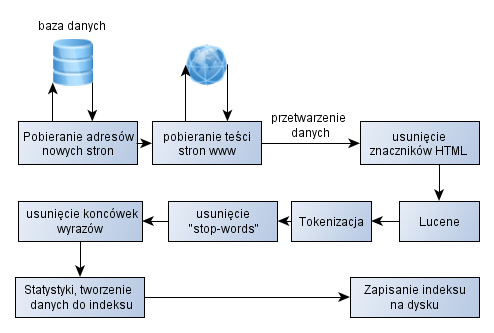
\includegraphics[width=1\textwidth]{lucene_indeksing.png}
\caption{Lucene: pobieranie danych i indeksowanie}
\label{fig:lucene_index_fig}
\end{figure}

We frameworku lucene zapisywana jest nie tylko treść strony www, ale również identyfikator dokumentu w bazie danych. W czasie wyszukiwania otrzymujemy jednocześnie informacje o rezultacie funkcji wyszukującej razem z odnośnikiem do dokumentu w bazie danych.



\subsection{Dane testowe}

W bazie danych znajdują się również dokumenty przeznaczone tylko do testowania skuteczności algorytmów. Dane te zostały pobrane ręcznie z różnych serwisów internetowych. Dzięki odmiennej tematyce tych stron internetowych, możemy założyć że dane te stanowią dwie odrębne grupy testowe:

\begin{itemize}
    \item PMC (http://www.ncbi.nlm.nih.gov/pmc/): zawierająca bazę artykułów z dziedziny medycyny. Pobrano 300 dokumentów.
    \item Arxiv: artykułów z dziedziny fizyki, astronomii i pokrewnych. Wybrano 146 artykulów.
\end{itemize}

Dane z bazy PMC można podzielić jeszcze na kilka poddziałów medycyny. Powstałe grupy to badania na temat chorób tarczycy, wirusy i AIDS. Ostatnie dwie grupy: wirusy i AIDS mogą się pokrywać. 

Każdemu dokumentowi zostały przydzielone odpowiednie etykiety. Utworzone zostały jako suma przydzielonych tagów przez autora tekstu i słów wchodzących w skład tytułu dokumentu.  Łączna ilość tagów przydzielona tym dokumentom wynosi 2856. 

Większość dokumentów pobranych z bazy PMC posiada informacje na temat ilości prac cytujących dany artykuł. Zostały one użyte jako ilość osób, które dodały dany dokument do bazy danych. Na potrzeby testów utworzono 198 użytkowników, których przyporządkowano do konkretnych dokumentów zgodnie z rozkładem normalnym. Dzięki temu wybrani użytkownicy charakteryzowali się zróżnicowaną aktywnością. 

Tagi, którymi użytkownik opisał dokument, są również losowane z przypisanego dla danego dokumentu zbioru. Dzięki temu każdy użytkownik, który dodał dokument mógł go opisać różnymi słowami kluczowymi.











